\section{Benchmarks}
\label{sec:benchmarks}
We ran various experiments to compare the different variants of the
algorithm C2 between themselves and to Lercier-Sirvent. All the
experiments were run on four dual-core Intel Xeon E5430 (2.6GHz),
eventually using the parallelized version of the algorithm.

\paragraph{Magma vs. \texttt{FAAST}}
\label{sec:magma-vs.-textttf}
The first set of experiments was run to evaluate the benefits of using
the algorithms of Chapter~\ref{cha:artin-schr-towers}. We selected
pairs of isogenous curves over $\F_{2^{101}}$ such that the height of
the tower is maximal (observe that this is always the case for
cryptographic curves).  We compared the Magma prototype to the
\texttt{FAAST}-based implementation of C2-AS-FI-MC using the
\texttt{zz\_p} and \texttt{GF2} data types (see
Section~\ref{sec:artin-benchmarks}).

\begin{figure}
  \centering
  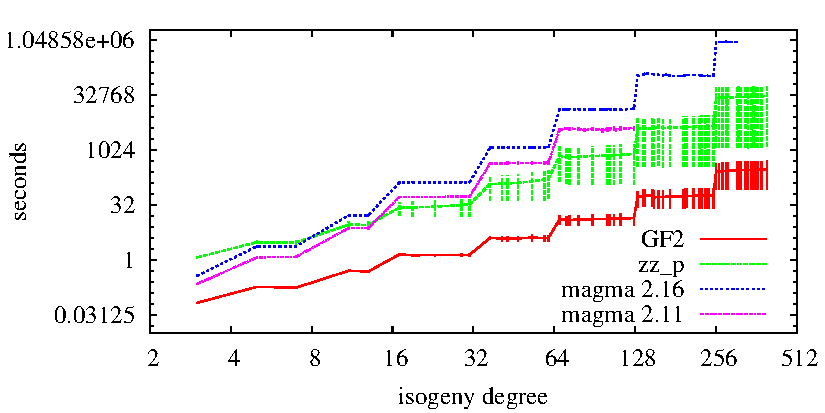
\includegraphics[width=0.9\textwidth]{isogeny/p2}
  \caption{Comparative timings for different implementations of C2-AS-FI-MC with curves defined over $\F_{2^{101}}$. Plot in logarithmic scale.}
  \label{fig:2-101}
\end{figure}

The results are in figure~\ref{fig:2-101}: we plot a line for the
average running time of the algorithm and bars around it for minimum
and maximum execution times of the final loop. Besides the dramatic
speedup obtained by using the ad-hoc type \texttt{GF2}, the
algorithmic improvements of \texttt{FAAST} over Magma are evident as
even \texttt{zz\_p} is one order of magnitude faster.

\begin{table}
  \centering
  \begin{tabular}{r r r r r r r r}
    \hline
    $\ell$ & $E[p^k]$ & $E'[p^k]$ & FI & RFR & MC & Avg tries & Avg loop time\\
    \hline
    31 & 1.3128 & 1.3128 & 1.1058 & 0.00218 & 0.00218 & 64 & 0.279\\
    61 & 3.5454 & 3.5464 & 2.5236 & 0.00783 & 0.00900 & 128 & 2.154 \\
    127 & 9.2975 & 9.3026 & 5.6881 & 0.03147 & 0.03634 & 256 & 17.359 \\
    251	& 23.7984 & 23.7984 & 12.7251 & 0.12415 & 0.14519 & 512 & 137.902 \\
    397 & 59.7439 & 59.7579 & 28.3387 & 0.36822 & 0.58027 & 1024 & 971.254 \\
    \hline
  \end{tabular}
  \caption{Comparative timings for the phases of C2-AS-FI-MC for curves over $\F_{2^{101}}$.}
  \label{tab:C2}
\end{table}

Table~\ref{tab:C2} shows detailed timings for each phase of
C2-AS-FI-MC. The column FI reports the time for one interpolation, the
column MC the time for one modular composition; comparing these two
columns the gain from passing from C2-AS-FI to C2-AS-FI-MC is
evident. Columns RFR (rational fraction reconstruction) and MC
constitute the Cauchy interpolation step that is repeated in the final
loop. The last column reports the average time spent in the loop: it
is by far the most expensive phase and this justifies the attention we
paid to FI and MC; only on some huge examples we approached the
crosspoint between these two algorithms.


\paragraph{C2-UD}
\label{sec:c2-ud}
Next we ran experiments on C2-UD. The first observation was that the
heuristic argument --on the probability that a degree sequence not
associated to an isogeny is not normal-- is well verified in practice:
except for a degree $2$ symmetry verified in characteristic $2$,
polynomials not associated to an isogeny very rarely gave a degree
sequence with a gap around the middle.

Looking for isogenies of unknown degree may be of some cryptographic
significance. For example, Teske's trapdoor cryptosystem selects a
binary field of composite degree ($\F_{2^{7\cdot 23}}$, in the
proposal) and chooses an elliptic curve $E$ vulnerable to the GHS
attack~\cite{gaudry+hess+smart02}. Then hides $E$ by taking a random
path of isogenies of small degrees landing on a curve $E'$ not
vulnerable to GHS, and uses $E'$ as public key. The security of the
cryptosystem comes from the assumption that it is infeasible to find a
GHS-vulnerable curve isogenous to $E'$, without the knowledge of the
isogeny path. 

The \emph{trapdoor} of the cryptosystem is the curve $E$: it is given
to a trusted authority so that --using an isogeny path from $E'$ to
$E$ and a GHS attack-- it has the power of deciphering messages at a
relatively high computational cost. This feature rests on the
assumption that it is feasible, but relatively hard, to compute any
isogeny path from $E$ to $E'$.


In this context, it may be interesting to verify that $E$ and $E'$ are
not relied by an isogeny of too low degree.
From~\cite[Appendix~A]{teske06}, we took the two curves defined over
$F_{2^{161}}=\F_2[z]/(z^{161}+z^{18}+1)$ of $j$ invariants:

$1/j = z^{152} + z^{143} + z^{139} + z^{136} + z^{135} + z^{133} +
z^{130} + z^{125} + z^{124} + z^{122} + z^{120} + z^{119} + z^{118} +
z^{117} + z^{116} + z^{114} + z^{113} + z^{112} + z^{110} + z^{109} +
z^{106} + z^{105} + z^{103} + z^{102} + z^{101} + z^{99} + z^{97} +
z^{96} + z^{92} + z^{91} + z^{88} + z^{87} + z^{86} + z^{85} + z^{81}
+ z^{78} + z^{77} + z^{76} + z^{75} + z^{73} + z^{71} + z^{69} +
z^{68} + z^{67} + z^{66} + z^{63} + z^{59} + z^{58} + z^{53} + z^{51}
+ z^{50} + z^{49} + z^{48} + z^{46} + z^{45} + z^{44} + z^{42} +
z^{38} + z^{34} + z^{3} + z^{32} + z^{31} + z^{29} + z^{27} + z^{26} +
z^{24} + z^{23} + z^{22} + z^{21} + z^{20} + z^{19} + z^{18} + z^{17}
+ z^{16} + z^{15} + z^{14} + z^{13} + z^{12} + z^{10} + z^{7} + z^{6}
+ z^{4} + z^{3} + z^{2}$,

$1/j'=z^{160} + z^{156} + z^{155} + z^{153} +z^{152} +z^{151} +z^{150}
+z^{149} +z^{148} +z^{147} +z^{146} +z^{145} +z^{143} +z^{142}
+z^{141} +z^{130} +z^{129} + z^{127} + z^{126} + z^{125} + z^{124} +
z^{123} + z^{120} + z^{118} + z^{112} + z^{109} + z^{104} + z^{103} +
z^{102} + z^{101} + z^{99} + z^{98} +z^{97} +z^{96} +z^{93} +z^{92}
+z^{91} +z^{90} +z^{88} +z^{85} +z^{83} +z^{77} +z^{74} +z^{70}
+z^{68} +z^{65} +z^{64} +z^{63} + z^{62} + z^{61} + z^{60} + z^{58} +
z^{57} + z^{55} + z^{50} + z^{48} + z^{45} + z^{41} + z^{38} + z^{37}
+ z^{36} + z^{33} + z^{31} + z^{30} + z^{27} +z^{26} +z^{24} +z^{23}
+z^{22} +z^{21} +z^{20} +z^{19} +z^{17} +z^{16} +z^{14} +z^{13}
+z^{10} +z^{8} +z^{7} +z^{4} +z^{3} +z$.

We ran our two variants of C2-UD on the two curves to certify the
conjectured property that no unexpected isogeny of low degree exists
between the two curves.

In 258 cpu-hours we were able to prove that no isogeny of degree
$p^c\ell$ for $\ell<2^{11}$ and $c$ arbitrary exists between the two
curves; in 1195 cpu-hours we were able to prove that no isogeny of
degree less than $2^{12}$ exists either. We stress the fact that,
albeit of little interest, this computation would have been impossible
without the (surprising) discovery of C2-UD.


\paragraph{Couveignes vs. Lercier-Sirvent}
Finally, we ran experiments on Lercier-Sirvent. Table~\ref{tab:ls}
shows timings for the different phases of the algorithm for some
isogeny degrees. The first column is the time spent to find a root of
$\Phi_\ell(X,j_E)$ in $\F_q$, the second column summarizes the time
spent to lift this root in $\Q_q$ and apply Elkies'
formulas. DiffSolve is the time spent solving the differential
equation, it is clearly the most expensive phase, although not the
most important asymptotically. RFR is the time for rational fraction
reconstruction, its rapid growth is justified by the fact that we
implemented it on top of a quadratic XGCD algorithm.

\begin{table}[ht]
  \centering
  \begin{tabular}{r r r r r r}
    \hline
    $\ell$ & Root $\Modpol_\ell$ & Elkies & DiffSolve & RFR & Other\\
    \hline
    31&1.49&0.50&12.15&0.35&0.08\\
    103&11.70&6.91&171.65&7.35&0.63\\
    149&21.77&17.43&427.08&18.53&1.31\\
    241&49.68&44.09&754.13&65.66&3.02\\
    331&79.43&126.21&1630.51&145.07&5.25\\
    397&101.04&176.23&1989.98&233.72&7.22\\
    \hline
  \end{tabular}
  \caption{Comparative timings for the phases of Lercier-Sirvent for curves over $\F_{5^{43}}$.}
  \label{tab:ls}
\end{table}


\begin{figure}
  \centering
  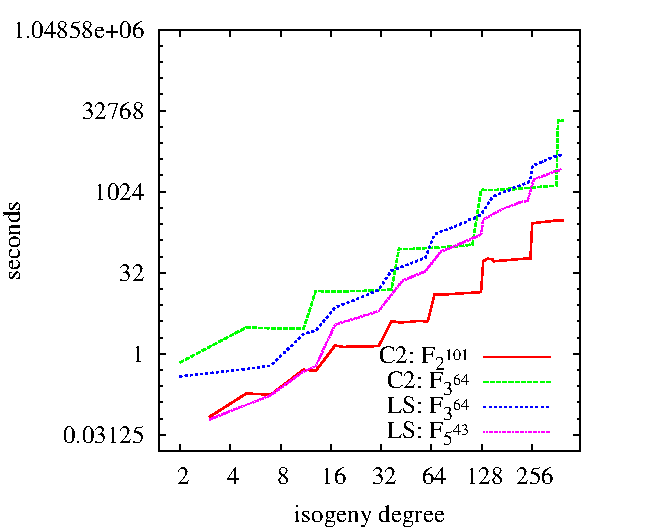
\includegraphics[height=0.45\textwidth]{isogeny/C2-LS}
  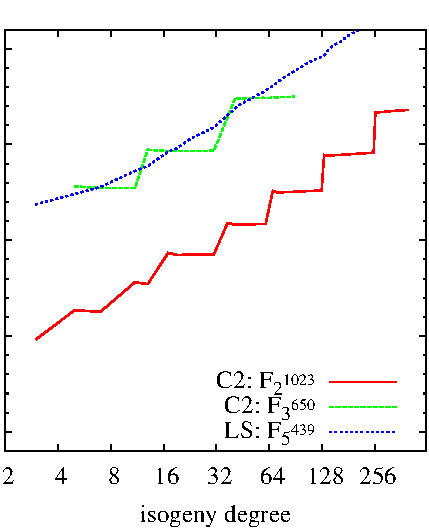
\includegraphics[height=0.45\textwidth]{isogeny/C2-LS2}
   \caption{Comparative timings for C2-AS-FI-MC (C2) and LS over
     different curves. Plot in logarithmic scale.}
  \label{fig:comp}
\end{figure}

We also compared the running times of C2-AS-FI-MC and LS over curves
of half the cryptographic size in figure~\ref{fig:comp} (left). We
only plot average times for C2, in characteristic $2$ we only plot the
timings for \texttt{GF2}. From the plot it is clear that C2-AS-FI-MC
only performs better than LS for $p=2$, but in this case Lercier's
algorithm~\cite{lercier96} is much faster.  Figure~\ref{fig:comp}
(right) shows that our implementation of LS slowly gets worse than C2,
however, comparing a Magma prototype to our highly optimized
implementation of C2-AS-FI-MC is somewhat unfair.

Furthermore, it is unlikely that C2-AS-FI-MC could be
practical for any $p>3$ because of its high dependence on $p$, while
LS scales pretty well with the characteristic as shown in
figure~\ref{fig:LSp}.

Considering that the asymptotic dependency of Couveignes' algorithm in
$\log q$ and in $p$ is worse than the one of Lercier-Sirvent (compare
Eq.~\eqref{eq:interp} to Proposition~\ref{th:lercier-sirvent}), there
are very few regions where Couveignes' algorithm stays of practical or
theoretical interest.

\pdfmargincomment{People don't like pessimism.}  Ironically, the
techniques presented in this document were developed in view of an
efficient implementation of Couveignes' algorithm, but, for the
moment, their only practical application seems to be C2-UD. Our hope
is that other interesting applications may be found in the future.

\begin{figure}
  \centering
  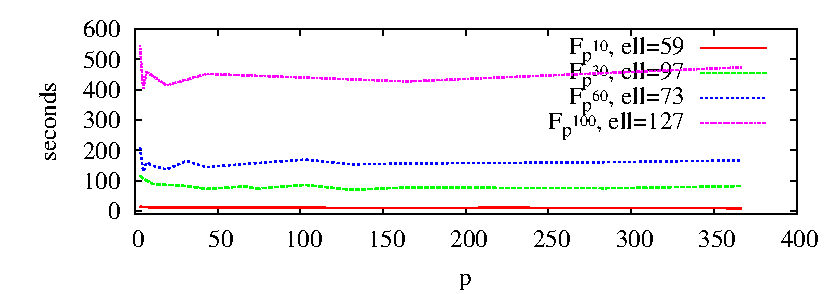
\includegraphics[width=0.9\textwidth]{isogeny/LSp}
  \caption{Timings for LS for different fields. We increase $p$ while
    keeping constant $d$ and the isogeny degree.}
  \label{fig:LSp}
\end{figure}


% Local Variables:
% mode:flyspell
% ispell-local-dictionary:"american"
% TeX-master: "../these"
% mode: TeX-PDF
% mode:reftex
% End:
%
% LocalWords:  Schreier Artin pseudotrace Frobenius bivariate Joux Sirvent FFT
% LocalWords:  Couveignes isogenies Schoof isogeny cryptosystems Lercier
% LocalWords:  precomputation arithmetics polylogarithmic Karatsuba precomputes
% LocalWords:  endomorphisms  isogenous
